%(BEGIN_QUESTION)
% Copyright 2006, Tony R. Kuphaldt, released under the Creative Commons Attribution License (v 1.0)
% This means you may do almost anything with this work of mine, so long as you give me proper credit

Studer følgende sløyfediagram:

$$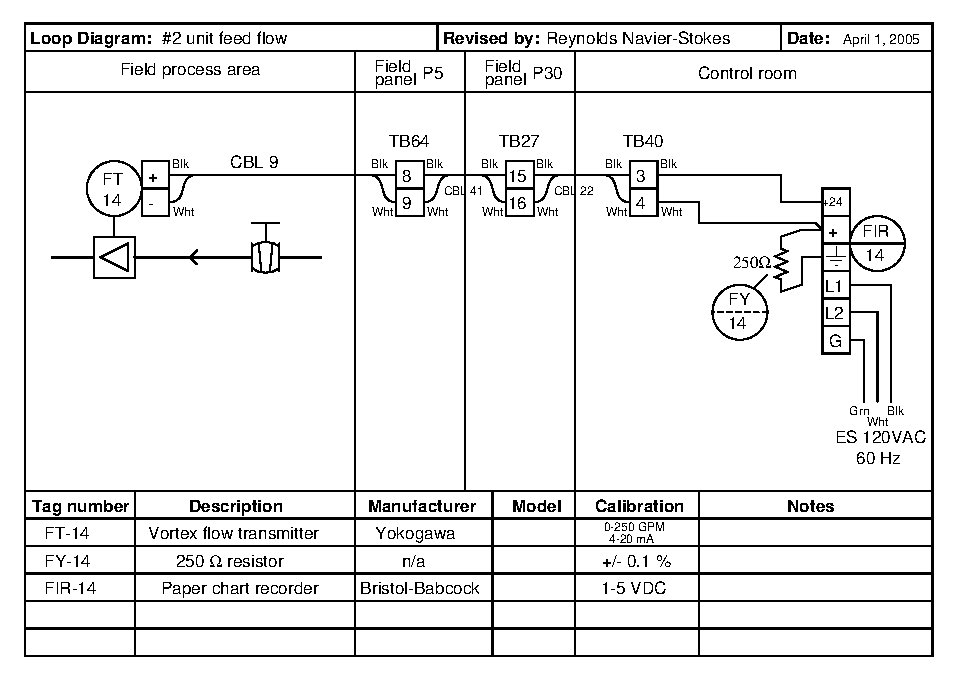
\includegraphics[width=15.5cm]{i00136x01.eps}$$

Følg strømveien i signalledningen, og bestem deretter følgende spenningsfall ved oppgitte strømningsrater. Anta en forsyningsspenning på nøyaktig 24 VDC:

\begin{itemize}
\item{} Spenning over FY-14-motstanden = \underbar{\hskip 50pt} ; Strømningsrate = 100 GPM
\item{} Spenning mellom terminal TB40-3 og TB40-4 = \underbar{\hskip 50pt} ; Strømningsrate = 200 GPM
\item{} Spenning over FT-14-senderterminalene = \underbar{\hskip 50pt} ; Strømningsrate = 175 GPM
\item{} Spenning mellom terminal TB64-8 og TB27-15 = \underbar{\hskip 50pt} ; Strømningsrate = 200 GPM
\end{itemize}

\underbar{file i00136}
%(END_QUESTION)





%(BEGIN_ANSWER)

$$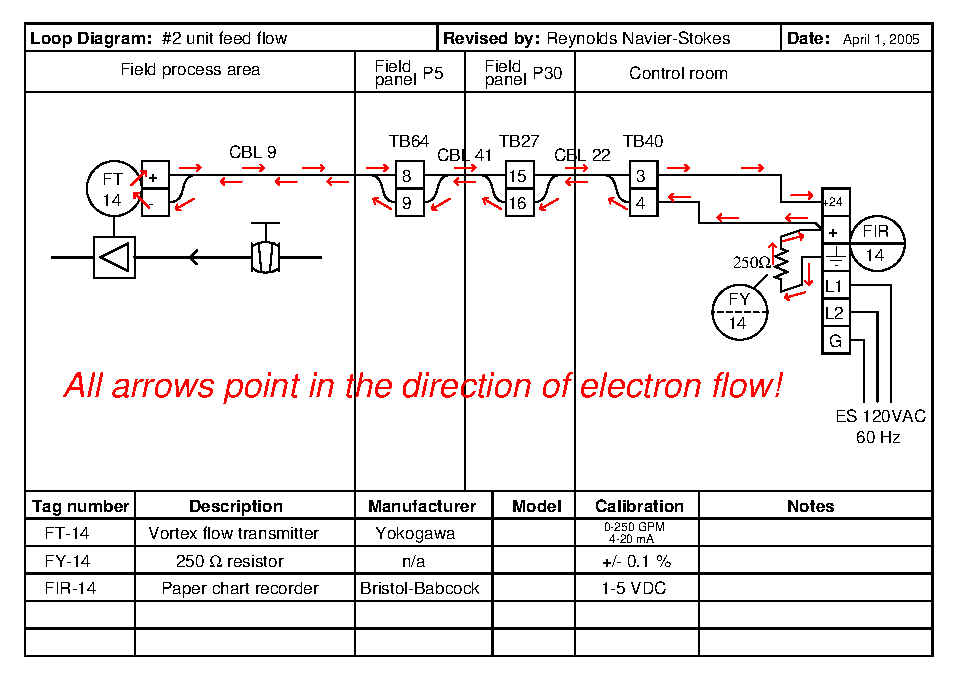
\includegraphics[width=15.5cm]{i00136x02.eps}$$

\noindent
{\bf Delvis svar:}

\begin{itemize}
\item{} Spenning over FY-14-motstanden = \underbar{\bf 2.6 volt} ; Strømningsrate = 100 GPM
\item{} Spenning mellom terminal TB40-3 og TB40-4 = \underbar{\bf 19.8 volt} ; Strømningsrate = 200 GPM
\item{} Spenning over FT-14-senderterminalene = \underbar{\hskip 50pt} ; Strømningsrate = 175 GPM
\item{} Spenning mellom terminal TB64-8 og TB27-15 = \underbar{\hskip 50pt} ; Strømningsrate = 200 GPM
\end{itemize}

%(END_ANSWER)





%(BEGIN_NOTES)

\begin{itemize}
\item{} Spenning over FY-14-motstanden = \underbar{\bf 2.6 volt} ; Strømningsrate = 100 GPM
\item{} Spenning mellom terminal TB40-3 og TB40-4 = \underbar{\bf 19.8 volt} ; Strømningsrate = 200 GPM
\item{} Spenning over FT-14-senderterminalene = \underbar{\bf 20.2 volt} ; Strømningsrate = 175 GPM
\item{} Spenning mellom terminal TB64-8 og TB27-15 = \underbar{\bf 0 volt} ; Strømningsrate = 200 GPM
\end{itemize}

\vskip 20pt \vbox{\hrule \hbox{\strut \vrule{} {\bf Virtuell feilsøking} \vrule} \hrule}

Dette spørsmålet egner seg godt som en «virtuell feilsøking»-øvelse. Når du presenterer diagrammet for studentene, ser du først for deg en bestemt feil i systemet. Deretter presenterer du ett eller flere symptomer på feilen (noe en operatør eller annen bruker kan observere). Studentene foreslår så diagnostiske tester for å finne feiltype og feilsted, som om de var teknikere i feilsøking. Din jobb er å oppgi hvilke resultater disse testene ville gitt, og dokumentere resultatene synlig for alle studentene.

Under og etter øvelsen er det nyttig å stille oppfølgingsspørsmål som:

\begin{itemize}
\item{} Hva forteller resultatet av siste diagnostiske test om feilen?
\item{} Anta at resultatet av siste test var annerledes. Hva ville det da fortalt om feilen?
\item{} Er siste diagnostiske test den beste vi kunne gjort?
\item{} Hva ville vært ideell testrekkefølge for å finne feilen i færrest mulig steg?
\end{itemize}

%INDEX% Basics, loop-powered transmitter: voltage drop calculations
%INDEX% Documentation, loop diagram

%(END_NOTES)
